\documentclass[12pt,utf8, 10pt]{article}
\usepackage[utf8]{inputenc}
\usepackage[german]{babel}
\usepackage{color}

\usepackage{graphicx}

\newcommand\svthema{Terminal Basics Cheat Sheet}
\newcommand\svperson{Jan-Marius Lenk, Christoph Parnitzke, Josef Schneider, Yannick Bungers}
\newcommand\svdatum{\today}
\newcommand\lvinst{Free and Open Source Software AG\\ Department of computer science}

\begin{document}
%TODO : title, author, etc
\date{\today}
\title{ \textbf{\color{blue}\svthema} }
\author{ \textsl{\color{black}\svperson} }
\date{ \small \lvinst \\ \svdatum}


\begin{figure}
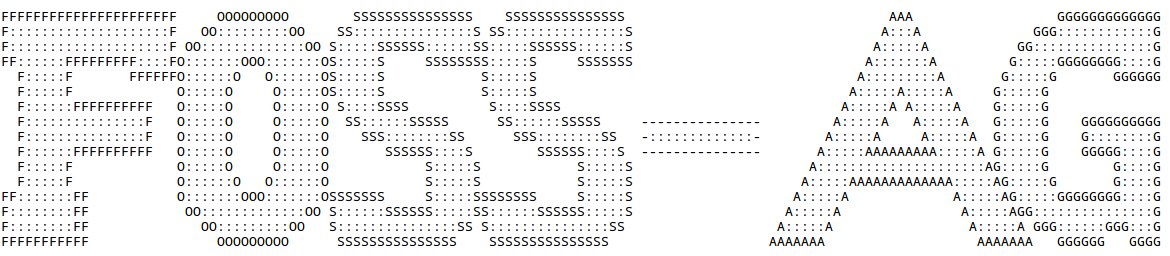
\includegraphics[scale=0.35]{foss-ag.png}
\end{figure}

\maketitle


\small
\textbf{Terminal vs. Shell}
\begin{itemize}
	\item Terminal: zeilenweise Eingabe von Befehlen
	\item TTY: Terminals via STRG+ALT+F[1-7]
	\begin{itemize}
		\item auch die grafische Oberfläche läuft auf einer Shell
		\item meist auf F7
	\end{itemize}
	\item VTerm: virtuelles Terminal in grafischer Umgebung
	\item Shell: interpretiert Benutzereingabe
\end{itemize}

\textbf{switch user}
\begin{itemize}
	\item Syntax: su [user]
	\item wechseln des Benutzers via Terminal
\end{itemize}


\twocolumn
%\center
\scriptsize
\textbf{super user do}
\begin{itemize}
	\item Syntax: sudo [command]
	\item ausführen von [command] mit erweiterten Rechten
	\item Parameter:
	\begin{itemize}
		\item -b (Ausführen von [command] im Hintergrund)
		\begin{itemize}
			\item Vorsicht bei interaktiven Programmen!!
		\end{itemize}
		\item -e (öffnet Datei zum editieren, erstellt tmp. Backup)
		\begin{itemize}
			\item gut beim Konfigurieren des Systems
			\item beugt Datenverlust vor
			\item Root wird neuer Besitzer der Datei
			\item statt 'sudo -e' 'sudoedit' möglich
		\end{itemize}
		\item -s (öffnet Shell)
		\item -u [user] (führt Befehl als [user] aus)
		\item -i (gibt root die .profile und .login des Benutzers)
		\begin{itemize}
			\item übergebene Befehle werden in Environment des Benutzers gestartet
			\item ohne '-c' wird interaktive Root-Shell geöffnet
		\end{itemize}
	\end{itemize}
\end{itemize}

\textbf{apt-get und aptitude}
\begin{itemize}
	\item immer mit 'sudo' ausführen
	\item apt statt apt-get möglich
	\item aptitude ist etwas grafischer und hat Zusatzfunktionen
	\item wichtigste Befehle:
	\begin{itemize}
		\item sudo apt install [pkg] ([pkg] installieren)
		\item sudo apt update (Datenbank der Pakete aktualisieren)
		\item sudo apt upgrade (mit Datenbank die Pakete aktualisieren)
		\item sudo apt dist-upgrade (wie upgrade, löst dependency Probleme)
		\item sudo apt remove [pkg] ([pkg] deinstallieren)
		\item sudo apt search [RegEx] (Paket suchen)
		\item sudo apt show [pkg] (zeigt Informationen zu [pkg])
		\item sudo apt list (zeigt Liste von Paketen)
		\item sudo apt list --installed (zeigt installierte Pakete)
	\end{itemize}
\end{itemize}

\textbf{man page}
\begin{itemize}
	\item Benutzerhandbuch des Systems
	\item Erklärung und sonstige Informationen zu installierten Paketen
	\item Sektionen:
	\begin{itemize}
		\item NAME (Name des Befehls)
		\item SYNOPSIS (Syntax des Befehls)
		\item CONFIGURATION
		\item DESCRIPTION (Beschreibung des Befehls)
		\item OPTIONS (Optionen, die beim Aufruf mit angegeben werden können)
		\item EXIT STATUS
		\item RETURN VALUE
		\item ERRORS
		\item ENVIRONMENT
		\item FILES
		\item VERSIONS
		\item CONFORMING TO
		\item NOTES
		\item BUGS (bekannte Fehler)
		\item EXAMPLE (Beispiele für den Aufruf)
		\item AUTHORS
		\item SEE ALSO
	\end{itemize}
	\item Suchverlauf
	\begin{itemize}
		\item[1.] ausführbare Programme und Shell Kommandos
        \item[2.] Systemaufrufe (vom Kernel bereitgestellt)
        \item[3.] Bibliotheksaufrufe (innerhalb von Programm-Bibliotheken)
        \item[4.] spezielle Dateien (in /dev)
        \item[5.] Dateiformate und Konventionen (/etc/passwd)
        \item[6.] Spiele
        \item[7.] Sonstiges (Macropakete und Konventionen)
        \item[8.] System administrations Kommandos (nur Root)
        \item[9.] Kernel Routinen (kein Standard)
	\end{itemize}
\end{itemize}

\textbf{list}
\begin{itemize}
	\item listet alle Dateien und Ordner im gegebenen Verzeichnis auf
	\item aktuelles Verzeichnis ist dabei Default
	\item Syntax: ls [option] [path]
	\item Parameter:
	\begin{itemize}
		\item -a (listet auch versteckte Dateien und Verzeichnisse)
		\item -l (listet auch Rechte, Besitzer, Gruppe, Größe, Name, last modified)
		\item -c (listet Zeit der letzten Modifikation)
		\item -f (gibt Inhalte in unsortierter Reihenfolge)
		\item -g (listet wie '-l' nur ohne Namen; '-G' ohen Gruppen)
		\item -h (gibt die Größe der Dateien für Menschen leserlicher aus)
		\item -m (gibt Liste durch Kommata getrennt)
		\item -r (reversive Auflistung der Inhalte)
		\item -R (rekursive Auflistung der Inhalte, auch Unterordner)
		\item -s (größe der Dateien)
		\item -1 (Auflistung zeilenweise)
		\item --sort=[var] (sortiert mit [var]=none (keine Sortierung); [var]=size (nach Größe sortiert); [var]=time (Sortierung nach Zeit); [var]=version (Sortierung nach Version), [var]=extension (Sortierung nach Anhang))
	\end{itemize}
\end{itemize}

\textbf{change directory}
\begin{itemize}
	\item Navigieren durch Dateisystem
	\item Syntax: cd [path]
	\item Wechsel in Parent-Directory '..' bzw. '../'
	\item Wechsel in Home-Directory 'cd' 
\end{itemize}

\textbf{make directory}
\begin{itemize}
	\item Erstellen von Verzeichnissen
	\item Syntax: mkdir [option] [path]
	\item Optionen:
	\begin{itemize}
		\item -p (erstellt Parent-Directory, falls es nicht existiert)
		\item -mode=[Mode] (Modus mit dem Ordner erstellt wird)
	\end{itemize}
\end{itemize}

\textbf{Gruppenverwaltung}
\begin{itemize}
	\item groups [user] (zeigt Gruppen von [user] an)
	\item groupadd [group] (legt Gruppe an) [nur Root]
	\item groupdel [group] (löscht Gruppe)  [nur Root]
	\item groupmod [option] [group] (modifizieren der Gruppen Eigenschaften) [nur Root]
	\item usermod -ag [user] [group] ([user] zu [group] hinzufügen) [nur Root]
	\item deluser [user] [group] ([user] aus [group] entfernen) [nur Root]
\end{itemize}

\textbf{change mode}
\begin{itemize}
	\item Ändern von Zugriffsrechte von Ordnern und Dateien
	\item Syntax: chmod [mode] [path]
	\item Elemente von [mode]:
	\begin{itemize}
		\item u= (Rechte des Besitzers)
		\item g= (Rechte der zugeordneten Gruppe)
		\item a= (Rechte aller anderer)
	\end{itemize}	 
	\item Rechte:
	\begin{itemize}
		\item r (Erlaubnis zum Lesen)
		\item w (Erlaubnis zum Schreiben)
		\item x (Erlaubnis zum Ausführen)
	\end{itemize}
\end{itemize}

\textbf{change owner}
\begin{itemize}
	\item Ändern des Besitzers und der Gruppe einer/s Datei/Ordners
	\item Benutzer ändern: chown [user] [file]
	\item Gruppe ändern: chown [user]:[group] [file]
	\item Parameter '-R' ändert Zugehörigkeit rekursiv
\end{itemize}

\textbf{remove directory}
\begin{itemize}
	\item Löschen von leeren Verzeichnissen
	\item Vorsicht: auch leere Verzeichnisse können wichtig sein
	\item leere Ordner in dem Ordner werden auch gelöscht
\end{itemize}

\textbf{echo}
\begin{itemize}
	\item Syntax: echo [option] [text]
	\item gibt eingegebenen Text wieder
	\item Ausnahme: echo \$c (gibt Wert von Variable 'c' aus)
	\item Parameter:
	\begin{itemize}
		\item -n (Ausgabe ohne neue Zeile)
		\item -e (Verwendung von Formatierungsoptionen)
	\end{itemize}
\end{itemize}

\textbf{stdin, stdout, stderr}
\begin{itemize}
	\item jeder Prozess hat 3 Datenströme
	\item stdin (Standard Input [number: 0])
	\item stdout (Standard Output [number: 1])
	\item stderr (Standard Error [number: 2])
\end{itemize}

\textbf{$<$, $>$ und Pipe}
\begin{itemize}
	\item Umleiten der Ein- und Ausgabe
	\item $<$ Laden der Eingabe aus Datei
	\item Syntax von $<$: [command] $<$ [path]
	\item $>$ Schreiben der Ausgabe in Datei
	\item Syntax von $>$: [command] $>$ [path]
	\item Pipe '$\mid$': [command1] $\mid$ [command2]
	\item Ausgabe von [command1] wird zu der Eingabe von [command2]
	\item stderr umleiten:
	\begin{itemize}
		\item '2$>$' es muss die Datenstromnummer angegeben werden
		\item Bsp. umleiten von stderr auf stdout:
		\item '[command] $>$ [path] 2$>\&$1'
	\end{itemize}	 
\end{itemize}

\textbf{more}
\begin{itemize}
	\item Filereader
	\item kein Editieren möglich
	\item Betrachten immer von oben nach unten
	\item Navigation ist etwas hinderlich
\end{itemize}

\textbf{less}
\begin{itemize}
	\item intelligenter Nachfolger von more
	\item unterstützt Scrolling
	\item Navigation:
	\begin{itemize}
		\item Pfeil- und Bildlauftasten
		\item '/pattern' durchsucht Dokument nach Muster
		\item '?pattern' wie '/pattern' nur umgekehrt
		\item '$\&$pattern' zeigt nur Zeilen mit Muster
		\item 'n' spring zum nächsten Mustervorkommen
		\item ':n' ruft nächste Dokument auf
	\end{itemize}
\end{itemize}

\textbf{concatenate}
\begin{itemize}
	\item konkateniert und zeigt Inhalte von Datei an
	\item Syntax: cat [option] [path]
	\item Optionen:
	\begin{itemize}
		\item -n (nummeriert ausgegebenen Zeilen)
		\item -s (unterdrückt Ausgabe von widerholenden Leerzeichen)
	\end{itemize}
\end{itemize}

\textbf{head und tail}
\begin{itemize}
	\item Textbetrachter auf bestimmte Bereiche der Datei
	\item \textbf{head} gibt ersten 10 Zeilen einer Datei aus
	\item \textbf{tail} gibt letzten 10 Zeilen einer Datei aus
	\item Parameter:	
	\begin{itemize}
		\item head [option] [path]
		\begin{itemize}
			\item -n [val] (gibt ersten [val] Zeilen aus)
		\end{itemize}
		\item tail [option] [path]
		\begin{itemize}
			\item -n [val] (gibt letzten [val] Zeilen aus)
			\item -f (gibt immer aktuelle Zeilen aus)
		\end{itemize}
	\end{itemize}
\end{itemize}

\textbf{Sortieren und Suchen}
\begin{itemize}
	\item Syntax: sort [option] [path]
	\begin{itemize}
		\item ließt Datei und sortiert Inhalt
		\item -r (Ausgabe umdrehen)
		\item -c (checkt ob Inhalt sortiert ist)
	\end{itemize}
	\item Syntax: find [option] [path] [pattern]
	\begin{itemize}
		\item sucht nach Dateien im System via Muster
		\item -m (sucht Dateiname, nicht Pfad)
	\end{itemize}
\end{itemize}

\textbf{copy und move}
\begin{itemize}
	\item Syntax:
	\begin{itemize}
		\item mv [path1] [path2]
		\item cp [path1] [path2]
	\end{itemize}
	\item Parameter:
	\begin{itemize}
		\item -i (fragt vor Überschreiben)
		\item -f (überschreibt \textbf{immer})
		\item -n (überschreibt \textbf{niemals})
		\item --backup (erstellt Backup vor Überschreiben
		\item -S, --suffix=[suf] (alternatives Suffix [suf] für Backup)
		\item -r (verschieben von Ordnern [nur 'cp'!!!!])
		\item -s (erstellt symbolische Links statt Dateien [nur 'cp' !!!!])
	\end{itemize}
\end{itemize}

\textbf{remove}
\begin{itemize}
	\item Löschen von Dateien und Ordnern
	\item Parameter:	
	\begin{itemize}
		\item -f (löschen ohne nachfragen)
		\item -i (Nachfragen bei jeder Löschung)
		\item -r (löscht rekursiv [für Ordner])
		\item -d (leere Verzeichnisse löschen)
	\end{itemize}
	\item 'rm' löscht nicht entgültig
\end{itemize}

\textbf{shred}
\begin{itemize}
	\item löscht Dateien entgültig
	\item Syntax: shred [option] [file]
	\item Parameter:
	\begin{itemize}
		\item -f (versucht Schreibrechte zu bekommen)
		\item -n [num] ([num] Schreibvorgänge pro Datei)
		\item -u (Löschung nach Überschreiben)
		\item -z (Nullen beim letzten Vorgang verwenden [Überschreiben verbergen])
	\end{itemize}
	\item Backups werden nicht mitgelöscht
\end{itemize}

\textbf{tar}
\begin{itemize}
	\item Syntax entpacken: tar [option] [path]
	\item Syntax verpackern: tar [option] [path-archiv] [path-files]
	\item Parameter:
	\begin{itemize}
		\item -c (erzeugt Archiv)
		\item -x (extrahiert Dateien)
		\item -v (Fortschritt auflisten)
		\item -z (komprimieren als .gz, etc.)
		\item -f (erzeugt beim entpacken einen Ordner mit Archivnamen)
		\item -j (bzip2 format)
		\item -r (Daten an Archiv anfügen)
		\item -d (Unterschiede zwischen 2 Archiven anzeigen)
	\end{itemize}
\end{itemize}

\textbf{Prozesse verwalten}
\begin{itemize}
	\item top:
	\begin{itemize}
		\item gehört zu Standardinstallation
		\item -h (Befehle anzeigen)
	\end{itemize}
	\item htop:
	\begin{itemize}
		\item meist nicht Standardinstallation
		\item leichtere Bedienung als 'top'
	\end{itemize}
	\item Optionen für 'htop':
	\begin{itemize}
		\item -d, --delay=[n] (Delay [n] zwischen Updates)
		\item -C, --no-color (htop ohne Farbe)
		\item -h (zeigt mögliche Optionen)
		\item -p, --pid=[PID1],[PID2],.. (zeigt nur Prozesse mit gegebener PID)
		\item -u, --user=[name] (zeigt nur Prozesse von Benutzer [name])
	\end{itemize}
	\item Ansicht:
	\begin{itemize}
		\item Auslastung einzelner CPU-Kerne und Arbeitsspeicher
		\item Anteil von Swap und bisherige Systemlaufzeit
		\item PID (Prozess-ID), User, PRI (Priorität), NI (Nice-Wert)
		\item VIRT und RES (benutzter virtueller und physischer Speicher)
		\item S (State; S $\in$ $\{$S[leeping], R[unning], D[ist sleep], Z[ombie], T[race/suspend], W[Paging]$\}$)
		\item CPU$\%$ und MEM$\%$ (genutzer CPU- und RAM-Anteil)
	\end{itemize}
\end{itemize}

\textbf{nice}
\begin{itemize}
	\item starten von Prozessen mit modifizierter Priorität
	\item -20 ist höchste, 19 ist niedrigste Priorität
	\item Syntax: nice [option] [command] [args]
	\item Parameter:
	\begin{itemize}
		\item -n, --adjustment=N (aufaddieren von N auf Nice-Wert)
	\end{itemize}
\end{itemize}

\textbf{ping}
\begin{itemize}
	\item prüft die Verfügbarkeit einer Adresse
	\item Syntax: ping [option] [addr] 
	\item -c [num] (Anzahl der Pings setzen)
\end{itemize}

\textbf{renice und nohup}
\begin{itemize}
	\item Syntax: renice [-n] priority [-g $\mid$ -p $\mid$ -u] identifier
	\begin{itemize}
		\item nachträglich den Nice-Wert eines Befehls einstellen
		\item -n [num] (neuer Nice-Wert)
		\item -g [group-id], -p [precess-id], -u [user-id]
	\end{itemize}
	\item Syntax: nohup [commando] [args]
	\begin{itemize}
		\item Programm läuft weiter auch nach Logout
	\end{itemize}
\end{itemize}

\textbf{$\&$}
\begin{itemize}
	\item Angabe am Ende von Prozess um diesen in Hintergrund zu verschieben
	\item stdout ist immernoch das Terminal
	\item Prozess blockiert Shell nicht
	\item \textbf{Achtung!!} $\&\&$ $\equiv$ Prozesse hintereinander ausführen
	\begin{itemize}
		\item p1 $\&\&$ p2 : p2 ausgeführt, wenn p1 erfolgreich
	\end{itemize}
\end{itemize}

\textbf{Texteditoren}
\begin{itemize}
	\item ed:
	\begin{itemize}
		\item nicht Teil der Standardinstallation
		\item erster Texteditor; Release: 1970
		\item a (append), i (insert), w (write), q (quit)
		\item Grundlage für grep
	\end{itemize}
	\item pico:
	\begin{itemize}
		\item Release: 1992
		\item sehr minimaltistischer Editor
		\item reine Textverarbeitung, mehrere Dokumente möglich, Syntaxhighlighting
		\item kein Highlighting von einem Wort, kein Text-Splitscreen, keine RegEx Suche 
	\end{itemize}
	\item nano:
	\begin{itemize}
		\item Release: 1999
		\item sehr minimaltistischer Editor
		\item Nachfolger von pico
		\item bietet mehr Funktionalität, z.B.: Text-Splitscreen, RegEx Suche
	\end{itemize}
	\item vim:
	\begin{itemize}
		\item Release: 1991
		\item Großmufti unter den Editoren
		\item verbesserte Suchfunktionen
		\item Standard bei 'git'
	\end{itemize}
	\item jed:
	\begin{itemize}
		\item Release: 1992
		\item Editor für Programmierer
		\item liefert Templates für verschiedene Anwendungsfälle
		\item weniger mächtig als vim
	\end{itemize}
\end{itemize}

\textbf{shutdown}
\begin{itemize}
	\item Ausschalten oder Neustart
	\item Syntax: shutdown [options] [time]
	\item Parameter:
	\begin{itemize}
		\item -P (poweroff)
		\item -r (reboot)
		\item -h (halt; kein Timer möglich)
	\end{itemize}
\end{itemize}

\textbf{ip addr}
\begin{itemize}
	\item Anzeigen von lokalen IP-Adressen
	\item Parameter:
	\begin{itemize}
		\item -4 Anzeigen der IPv4-Adressen
		\item -6 Anzeigen der IPv6-Adressen
	\end{itemize}
\end{itemize}

\textbf{nmon}
\begin{itemize}
	\item Shortcuts:
	\begin{itemize}
		\item c (zeigt Auslastung aller CPU Kerne)
		\item m (zeigt Auslastung Arbeitsspeicher [mit Swap])
		\item d (zeigt Auslastung der Festplatte)
		\item k (zeigt Kernel Statistiken)
		\item r (Details zum System und Prozessor)
		\item l (CPU Auslastung als Graph)
		\item n (Auslastung der Netzwerk Schnittstellen)
		\item j (Auslastung des Dateisystems)
		\item t (wie top, alle laufenden Prozesse)
		\item + bzw. - (Refresh erhöhen bzw. verringern)
		\item H (Hilfe)
	\end{itemize}
\end{itemize}

\textbf{RegEx}
\begin{itemize}
	\item zeigen Grundstruktur von gesuchtem Begriff
	\item Angeben immer in Anführungszeichen
	\item Syntax:
	\begin{itemize}
		\item c (konstantes Zeichen c)
		\item . (genau \textbf{ein} beliebiges Zeichen)
		\item .* (Folge von beliebigen Zeichen [auch keines])
		\item * (Zeichen vor * ist beliebig oft [auch gar nicht])
		\item ? (Zeichen vor ? ist \textbf{genau} einmal oder gar nicht)
		\item + (Zeichen vor + min. einmal)
		\item $\{$n,m$\}$ (Zeichen wird n bis m mal wiederholt)
		\item $\{$n$\}$ (Zeichen wird genau n mal wiederholt)
		\item '[...]' (Zeichen kommt in den Klammern vor) [Hochkommata ignorieren]
		\item '[...-...]' (Zeichen ist aus Zeichenklasse) [Hochkommata ignorieren]
		\item '[$\hat{}$...]' und [$\hat{}$...-...] (verneinen von Zeichenklasse) [Hochkommata ignorieren]
		\item \$ (Zeilenende)
		\item $<$ (Wortanfang)
		\item $>$ (Wortende)
		\item a1$\mid$a2 (alternative Ausdrücke; a1 oder a2)
		\item (...) Gruppe von Ausdrücken
		\item $\setminus$ Sonderbedeutung von nächstem Symbol ignorieren
	\end{itemize}
\end{itemize}

\textbf{grep}
\begin{itemize}
	\item durchsucht eine Eingabe nach einem RegEx
	\item Syntax: grep [path] [RegEx]
	\item Selektoren:
	\begin{itemize}
		\item -E (Interpretiert Suchwort als erweiterten RegEx)
		\item -F (Interpretiert Suchwort als fixed String)
		\item -G (Interpretiert Suchwort als basic RegEx)
	\end{itemize}
	\item Kontrolle:
	\begin{itemize}
		\item -f [file] (liest RegEx aus [file])
		\item -v (invertiert das Matchmaking)
		\item -w (gibt nur Zeilen aus, in denen ganze Worte dem RegEx entsprechen)
		\item -x (gibt nur Zeilen aus, die ganz dem RegEx entsprechen)
	\end{itemize}
	\item Ausgabe:
	\begin{itemize}
		\item -c (gibt Anzahl der passenden Zeilen aus)
		\item -o (gibt nur gematchten Teile einer Zeile aus)
		\item -q (keine Ausgabe, gibt Exitcode 0 aus, falls erfolgreich)
	\end{itemize}
\end{itemize}

\textbf{Alias}
\begin{itemize}
	\item Setzen von Alias für einen Befehl
	\item Vorgehen:
	\begin{itemize}
		\item Bearbeite ~/.bashrc
		\item füge \texttt{alias [aliasname]='[Befehl]'} hinzu
		\item speichern
		\item neu einloggen oder \texttt{source ~/.bashrc}
	\end{itemize}
	\item Bsp. Zeile: alias ll='ls -l'
\end{itemize}
\end{document}
